% =============================================================================
% cs-linked-list.tex — Singly linked list with data/next cells and NULL terminator
%
% Shows: three nodes, each split into a data field and a next-pointer field,
% with arrows from each next field to the following node and a NULL slash on
% the last. A `head` pointer points at the first node.
% Compiles standalone via: xelatex cs-linked-list.tex
%
% Use for: data structures (linked lists, stacks/queues by linking), pointers
% and dynamic memory, insert/delete pointer-rewiring diagrams.
%
% To show an INSERT: draw the new node below the list and re-route one arrow;
% keep the old arrow in `muted` dashed to show what is being replaced.
% =============================================================================

\documentclass[border=4pt]{standalone}
\usepackage{tikz}
\usetikzlibrary{arrows.meta, positioning, calc}

\definecolor{cell-fill}{HTML}{E8EDF5}
\definecolor{cell-border}{HTML}{012169}
\definecolor{ptr}{HTML}{B9975B}
\definecolor{muted}{HTML}{525252}

\tikzset{
  datacell/.style={
    draw=cell-border, fill=cell-fill, thick,
    minimum width=1.0cm, minimum height=0.9cm, align=center, font=\small
  },
  nextcell/.style={
    draw=cell-border, fill=white, thick,
    minimum width=0.7cm, minimum height=0.9cm, align=center, font=\small
  },
  ptr-edge/.style={-{Latex[length=2.4mm]}, thick, draw=ptr},
  lbl/.style={font=\scriptsize, text=muted}
}

% -----------------------------------------------------------------------------
% Diagram: head -> [10|*] -> [20|*] -> [30|/]
% Coordinates: (x, y) — each node is a data cell + a next cell, drawn as two
% abutting rectangles so the boundary between fields is visible.
%   Node 1 data at (0.0, 0); next at (0.85, 0)
%   Node 2 data at (3.4, 0); next at (4.25, 0)
%   Node 3 data at (6.8, 0); next at (7.65, 0)
% Cell widths: data 1.0, next 0.7 -> they abut exactly at 0.85 = 0.0+0.5+0.35.
% Pointer arrows leave the RIGHT edge of a next cell and enter the LEFT edge of
% the following data cell: a 2.15cm clear span, so arrowheads never touch a box
% (P7a). The `head` label sits ABOVE its arrow, not on it (P7b).
% -----------------------------------------------------------------------------

\begin{document}
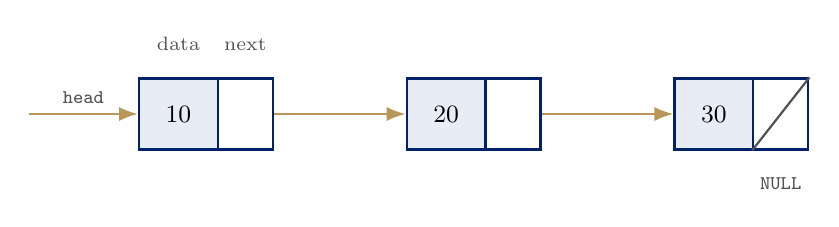
\begin{tikzpicture}

  % ---- Node 1 --------------------------------------------------------------
  \node[datacell] (d1) at (0.00, 0) {10};
  \node[nextcell] (n1) at (0.85, 0) {};

  % ---- Node 2 --------------------------------------------------------------
  \node[datacell] (d2) at (3.40, 0) {20};
  \node[nextcell] (n2) at (4.25, 0) {};

  % ---- Node 3 --------------------------------------------------------------
  \node[datacell] (d3) at (6.80, 0) {30};
  \node[nextcell] (n3) at (7.65, 0) {};

  % ---- head pointer --------------------------------------------------------
  \draw[ptr-edge] (-1.9, 0) -- node[above, lbl] {\texttt{head}} (d1.west);

  % ---- next pointers -------------------------------------------------------
  \draw[ptr-edge] (n1.east) -- (d2.west);
  \draw[ptr-edge] (n2.east) -- (d3.west);

  % ---- NULL terminator: diagonal slash through the last next cell ---------
  \draw[thick, draw=muted] (n3.south west) -- (n3.north east);
  \node[lbl, below=0.22cm of n3] {\texttt{NULL}};

  % ---- Field legend --------------------------------------------------------
  \node[lbl, above=0.22cm of d1] {data};
  \node[lbl, above=0.22cm of n1] {next};

\end{tikzpicture}
\end{document}
